\section{Structure}
In this section we will be describing the overall structure of the program, through class diagrams.

\subsection{Individual class description}\fxnote{Remove some of this shit..}
The \textbf{Foodplan} class describes a schedule of planned meals that a user can administrate and follow.
It can consists of 0 to many meals.

The \textbf{Meal} class contains information about a meal and when to make/eat it. It consists of recipes.

\textbf{Recipes} consists of \textbf{Food}.

\subsection{Class diagram description}
The class diagram is structured with \textbf{Food} as the central class. 
\textit{Shopping List}, \textit{Inventory} and \textit{Foodplan} are lists, containing \textit{Food} or \textit{Meal}.

Food objects can be part of a \textbf{Shopping List}, a user \textbf{Inventory}, or be part of a \textbf{Recipe}, seen as aggregation on \cref{fig:classDiagram}. A \textbf{Recipe} contains 1 to many Food objects, and is part of a \textbf{Meal} that in turn is part of a \textbf{Foodplan}. A \textit{Meal} contains exactly 1 recipe, while the \textit{Foodplan} can have any number of planned \textit{Meals}.

\fxnote{fix references..}
\begin{figure}[H]
	\centering
	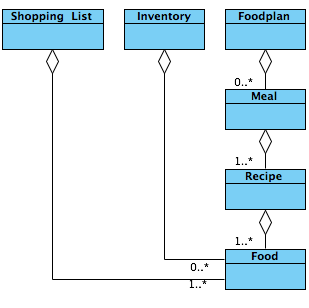
\includegraphics[width=0.50\textwidth]{Grafik/FoodPlanner/FoodPlannerClassDiagram.png}
	\caption{Relation between classes.}
	\label{fig:classDiagram}
\end{figure}

\fxnote{Update diagram to anders super-style with attributes}
